\providecommand{\relativeRoot}{../..}
\documentclass[\relativeRoot/main.tex]{subfiles}
\graphicspath{{\subfix{./figures/}}}


\begin{document}

\section{Documentation}
\label{sec:lyprox:documentation}

\begin{figure}
    \centering
    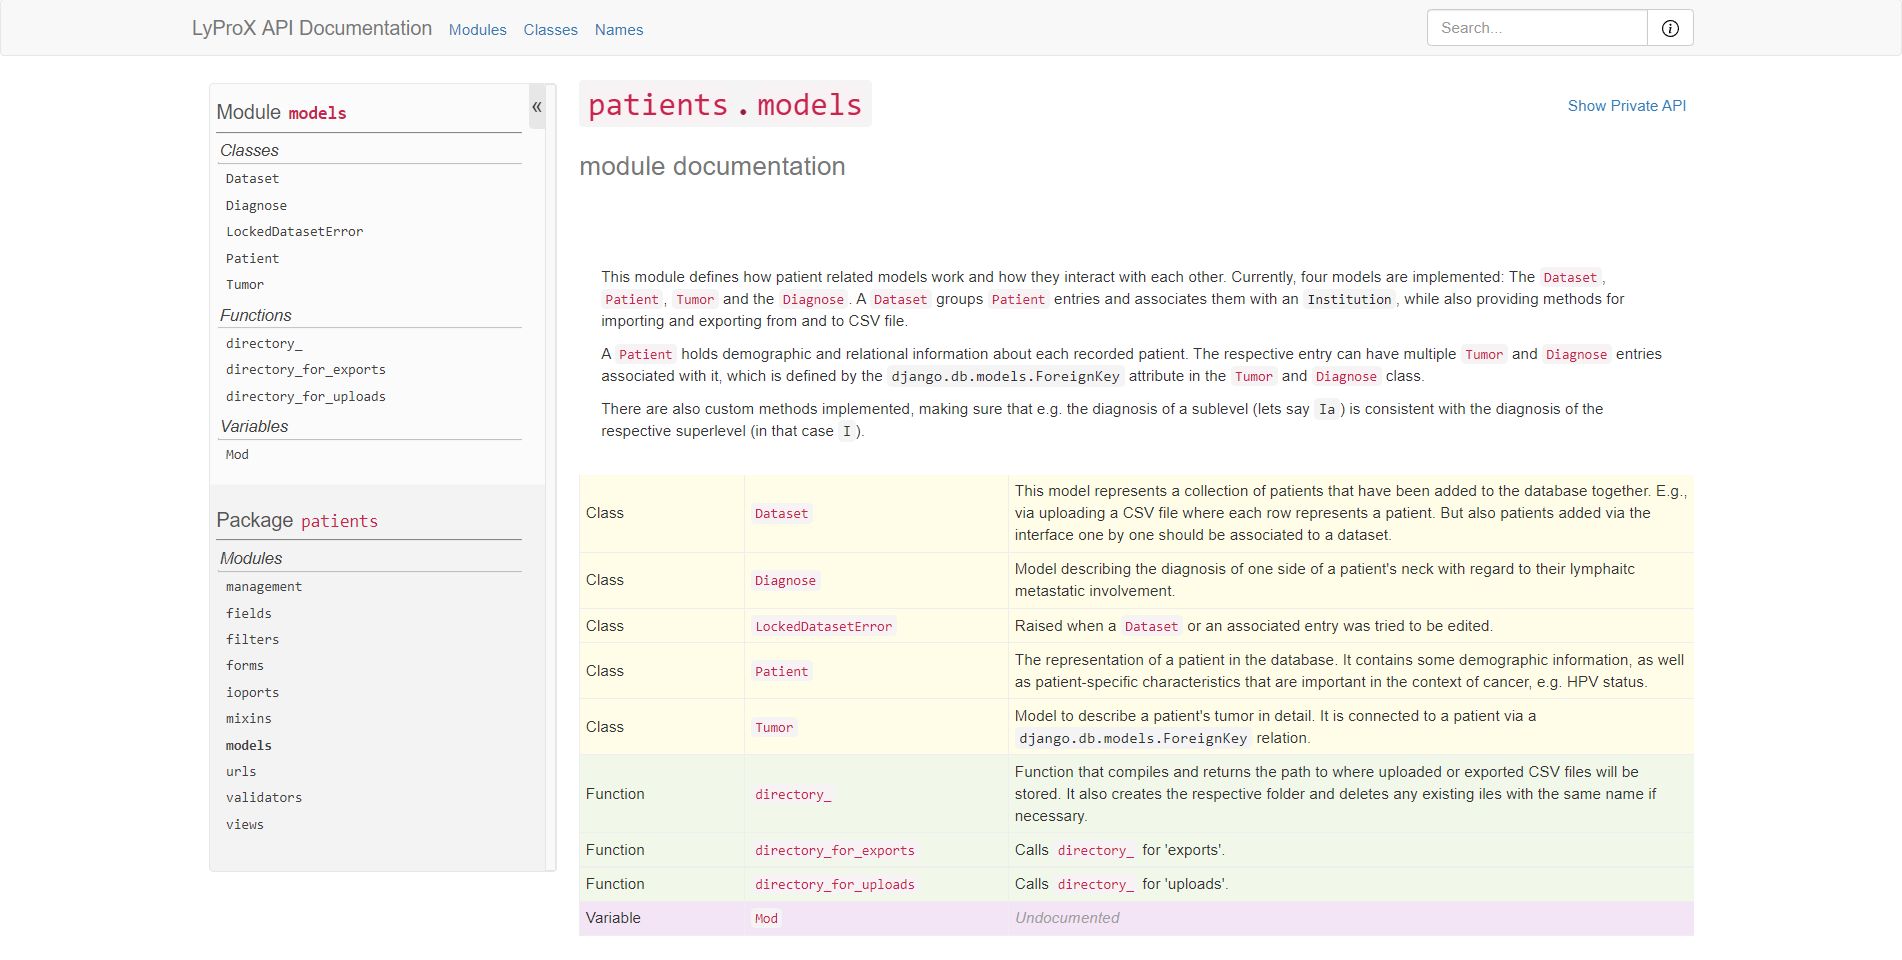
\includegraphics[width=\textwidth, frame]{figures/docs.png}
    \caption[
        Documentation for LyProX
    ]{
        Screenshot of a part of the \acrshort{api} documentation for LyProX. The displayed page documents the patient related model classes that represent SQLite3 database tables. It is auto-generated by \texttt{pydoctor} \cite{hudson_pydoctor_2022} using static code analysis.
    }
    \label{fig:lyprox:documentation}
\end{figure}

To improve the maintainability of the implementation, we decided to automatically build a documentation from the docstrings in LyProX' source code and make it available alongside the GitHub repository.

Since a Django app cannot be executed or imported like a standalone Python module, dynamic auto-generation of documentation is cumbersome to set up and error-prone. Hence, we resorted to a tool called \href{https://pydoctor.readthedocs.io/en/latest/}{\faIcon{external-link-alt}~\texttt{pydoctor}} \cite{hudson_pydoctor_2022} that statically analyses code for docstrings without importing or executing anything. Consequently, very little configuration is necessary to generate an informative static webpage containing information on the internal \acrshortpl{api}.

Like the deployment, building the documentation and hosting it is performed automatically -- using \href{https://github.com/features/actions}{\faIcon{external-link-alt}~GitHub actions} -- whenever a new version is merged into the \texttt{main} branch of the development repository \repolink{lyprox}. Subsequenty, the built documentation that \texttt{pydoctor} outputs is hosted on \href{https://pages.github.com/}{\faIcon{external-link-alt}~GitHub pages} under the URL \href{https://rmnldwg.github.io/lyprox}{\faIcon{external-link-alt}~\texttt{rmnldwg.github.io/lyprox}}. A screenshot of it is shown in \cref{fig:lyprox:documentation}.

At the time of writing this thesis, the documentation is in a very basic state. It essentially only collects and nicely displays how we have documented the source code. However, in the future we intend to extend this substantially and make it a comprehensive guide, aiding potential collaborators in understanding how LyProX is built and thus make contributing to it easier. Moreover, as the scope and complexity of the project grows, we ourselves might need to depend on a well-written documentation so that adding new features remains smooth and not unnecessarily time-consuming.

\end{document}
